%%%%%%%%%%%%%%%%%%%%%%%%%%%%%%%%
% DOSSIER DE CONCEPTION        %
%%%%%%%%%%%%%%%%%%%%%%%%%%%%%%%%
% définition et packages du présent fichier
%%%%%%%%%%%%%%%%%%%%%%%%%
% PACKAGES              %
%%%%%%%%%%%%%%%%%%%%%%%%%
\documentclass{report}
\usepackage[utf8x]{inputenc}  % accents
\usepackage{geometry}         % marges
\usepackage[francais]{babel}  % langue
\usepackage{graphicx}         % images
\usepackage{verbatim}         % texte préformaté
\usepackage{fancyhdr}         % fancy






% Titre de ce fichier dans le fancy 
\newcommand{\titre}{{\Huge Dossier de conception}\\Groupe B}
\newcommand{\titrehead}{Dossier de conception}
% Inclusion du préambule commun
%%%%%%%%%%%%%%%%%%%%%%%%%
% PRÉAMBULE             %
%%%%%%%%%%%%%%%%%%%%%%%%%
\title{\titre{}}
\author{}
% laisser vide pour date de compilation
\date{} 

% FORMAT PAGES         
\pagestyle{fancy} % nom du rendu (définit les lignes suivantes)
        \lhead{} % left head
        \chead{\titrehead{}} % center head
        \rhead{} % right head
        \lfoot{} % left foot
        \cfoot{\thepage} % center foot
        \rfoot{} % right foot


% Ce fichier est un préambule commun à toutes les sources LaTeX.
% Il est inclus par toutes les sources et permet d'avoir un formatage commun facilement modifiable.




%%%%%%%%%%%%%%%%%%%%%%%%%
% BEGIN                 %
%%%%%%%%%%%%%%%%%%%%%%%%%
\begin{document}
\maketitle
\tableofcontents



%%%%%%%%%%%%%%%%%%%%%
% CHAPTER 1         %
%%%%%%%%%%%%%%%%%%%%%

\chapter{Introduction}


\section{Présentation du document}
        \paragraph*{}
        Ce document présente le dossier de conception du projet « PicrossProject ». Il a pour
	but de décrire précisément les outils et langages utilisés pour la conception.
	Ce document fait référence au Cahier des Charges du projet qui définit les
	besoins du client, ainsi que les différentes fonctionnalités de l’application souhaitée.

\section{Contexte}
        \paragraph*{}
        Le présent document explicite l’architecture, les renseignements techniques
	ainsi que les contraintes à prendre en compte pour le développement de
	l’application.
	Il a pour but de définir le produit, de détailler sa conception afin qu’il soit
	conforme à la conception validée par le chef de projet et aux attentes du client.



\section{Portée du document}
        \paragraph*{}
        Il est destiné :
            \begin{itemize}
                \item aux enseignants du département Informatiques évaluant les produits de ce projet;
                \item à l'équipe du projet lors du développement du produit.
            \end{itemize}    
            
           Il servira de base :
            \begin{itemize}
                \item à l'évaluation du produit final;
                \item au développement des différents modules.
             \end{itemize}
             

\section{Équipe de développement}
        \paragraph*{}
        Le travail d'implémentation, de documentation du code et de rédaction/maintenance des documents sera divisé entre les développeurs.
        
        \begin{itemize}
                \item Charlie Maréchal (documentaliste, développeur Moteur);
                \item Ewen Cousin (développeur GUI);
                \item Jaweed Parwany (développeur Aide);
                \item Julien Le Gall (développeur Aide);
                \item Lucas Bourneuf (chef d'équipe, développeur Moteur);
                \item Nicolas Bourdin(développeur GUI);
        \end{itemize}
             



%%%%%%%%%%%%%%%%%%%%%
% CHAPTER 2         %
%%%%%%%%%%%%%%%%%%%%%
\chapter{Présentation du projet}
\section{Contexte }
        \paragraph*{}
	Le projet à été proposé par les enseignants du département informatique de l'Université du Maine du Mans 
	dans le cadre du module Projet en Génie Logiciel.
	Aucun outils de developpement n'est imposé, le groupe doit donc s'organiser de la façon qui lui semblera la plus pratique. 
	Le réalisation du projet se fera uniquement grace à l'utilisation des moyens fournis par l'université ainsi qu'avec le matériel dont 
	disposent personnellement les étudiants memebres du groupe. 


\section{Objectifs}
\paragraph*{}


\subsection{Critères d'acceptabilité du produit}
        \paragraph*{}
	L’application doit répondre aux critères suivants :
	\begin{itemize}
  	  	\item validation du produit via un dossier de tests réalisés par notre groupe;
  	  	\item respect des choix technologiques du client (cf. "Contraintes techniques");
  	  	\item respect des contraintes client (cf. "Contraintes client");
	\end{itemize}



%%%%%%%%%%%%%%%%%%%%%
% CHAPTER 3         %
%%%%%%%%%%%%%%%%%%%%%
\chapter{Environnements et outils de développement} 


\section{Éditeurs \& outils de développement}
        \paragraph*{}
        Aucun éditeur particulier n'a été imposé à l'équipe, si bien que les  développeurs ont utilisés chacun leur solution favorite, telles que :
	\begin{itemize}
		\item vim;
		\item kate;
		\item sublim text 2.
	\end{itemize}
	\paragraph*{}
	Le code ayant été forgé sous une seule architecture (UNIX), aucun problème de compatibilité n'a entaché la forge.
	\paragraph*{}
	L'automatisation des tâches de compilation et interprétation a été confié à \textit{make}.


\section{Conventions}
        \paragraph*{}
        Afin de garantir une homogénéité du code final, des conventions sont appliquées par l'ensemble des développeurs.
	\begin{itemize}
		\item  la tabulation est opérée avec deux espaces\footnote{Convention  globablement observées, notamment dans le code de \textit{Ruby On  Rails}};
		\item le code est documenté suivant les standards de rdoc\footnote{Dont l'usage est détaillé via http://rdoc.rubyforge.org/};
		\item écriture des identificateurs en camlCase, des noms de classe débutant par une majuscule.
		%\item ;
	\end{itemize}


\section{Coworking over IP}
        \paragraph*{}
         Afin de coordonner l'équipe avec la même efficacité que durant les séances de projet, plusieurs outils de \textit{coworking over IP} ont  été utilisés.
Ces outils ont permis un travail collaboratif essentiel à la réalisation du projet, notamment les parties de mise en commun du code.
        \begin{itemize}
                \item git;
                \item Github\footnote{http://github.com};
                \item Etherpad\footnote{http://etherpad.org}, dont une instance à été fournie par le HAUM\footnote{http://haum.org};
        \end{itemize}






%%%%%%%%%%%%%%%%%%%%%%
% CHAPTER 4          %
%%%%%%%%%%%%%%%%%%%%%%
\chapter{Architecture logicielle}


\section{Organisation des sources}
        \paragraph*{}
   Les sources ont été organisées en ces différents modules :
    \begin{itemize}
             \item commun, qui contient les constantes, et les classes de bases(Etat, etc..);
             \item configuration, qui enregistre les valeurs pour la configuration du programme et son fonctionnement interne;
             \item grille, qui contient les différentes classes de grilles;
             \item picross, la classe principale utilisant les autres modules pour produire le programme final;
             \item gui, la classe exploitant GTK2 pour gérer l'interface graphique;
             \item image, pour la transformation d'une image en grille de picross;
             \item scores, référençant les scores selon les grilles et les joueurs;
             \item gestionnaire, les classes gérant les sauvegardes et la persistance des données relatives aux grilles. % A CODER
        \end{itemize}
        
        \paragraph*{}
        Le fichier \textit{main.rb} contient le code utilisateur de la classe picross. Utiliser l'interpréteur sur ce fichier lance le programme dans  sa totalité.
	Aucun argument n'est attendu.

\section{Diagramme de classe}
        \paragraph*{}
 
 	\begin{center}
        	\includegraphics[scale=0.6]{data/umlDiagram.jpg}\\
        	\textbf{Diagramme UML}
	\end{center}
        


\section{Persistance des données}
        \paragraph*{}
         Trois types de données principaux persisteront sur le système utilisateur. Aucun fichier ne devrait être modifié par l'utilisateur.
        \begin{itemize}
		\item Le programme nécessite l'enregistrement de certaines données, telles que l'id de grille non assigné le plus petit.
		Ces données sont conservées et enregistrées dans le module Configuration.
		\item Les grilles racines utilisées par l'utilisateur sont sauvegardées localement pour être facilement accessible 
		et modifiables par le programme, à l'aide du gestionnaire de grille racine.
		\item Les grilles sauvegardées par l'utilisateur sont conservées et gérées à l'aide du gestionnaire de sauvegarde.
        \end{itemize}



%%%%%%%%%%%%%%%%%%%%%%
% CHAPTER 4          %
%%%%%%%%%%%%%%%%%%%%%%
\chapter{Maquette IHM}


 %\begin{center}
                %\includegraphics[scale=0.6]{data/Nouvelle Grille.png}\\
                %\textbf{Nouvelle Grille}
%\end{center}

 %\begin{center}
                %\includegraphics[scale=0.6]{data/Fenetre Edition.png}\\
                %\textbf{Fenetre Edition}
%\end{center}

 %\begin{center}
                %\includegraphics[scale=0.6]{data/Edition Grille.png}\\
                %\textbf{Edition Grille}
%\end{center}

 %\begin{center}
                %\includegraphics[scale=0.6]{data/Charger Image.png}\\
                %\textbf{Charger Image}
%\end{center}

 %\begin{center}
                %\includegraphics[scale=0.6]{data/Charger Grille.png}\\
                %\textbf{Charger Grille}
%\end{center}

 %\begin{center}
                %\includegraphics[scale=0.6]{data/Sauvegarde Grille.png}\\
                %\textbf{Sauvegarde Grille}
%\end{center}

 %\begin{center}
                %\includegraphics[scale=0.6]{data/umlDiagram.jpg}\\
                %\textbf{Diagramme UML}
%\end{center}

 %\begin{center}
                %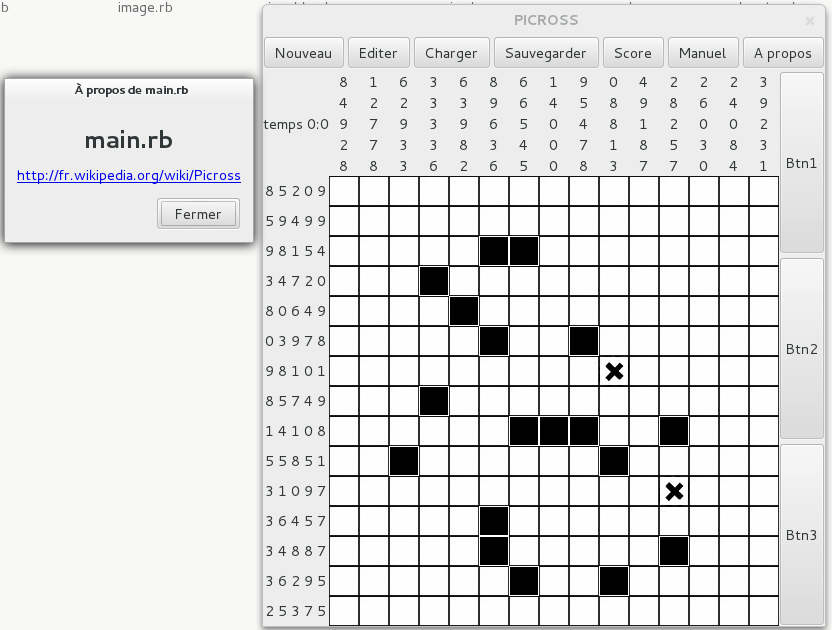
\includegraphics[scale=0.6]{data/Manuel.png}\\
                %\textbf{Manuel}
%\end{center}

 %\begin{center}
                %\includegraphics[scale=0.6]{A Propos.png}\\
                %\textbf{A Propos}
%\end{center}


\end{document}
% END
